\documentclass[12pt,a4paper]{article}
\usepackage{vntex} % Tiếng Việt
\usepackage{graphicx} % Chèn hình ảnh
\usepackage{fancyhdr} % Gói hỗ trợ tạo header và footer fancy
\usepackage{changepage} % Thay đổi lề

% Chèn code
\usepackage{listings} % Thêm gói listings để chèn code
\usepackage{xcolor} % Màu cho code
\lstset{
    language=R,
    basicstyle=\footnotesize\ttfamily,
    numbers=none,
    numberstyle=\tiny\color{gray},
    stepnumber=1,
    numbersep=0.01pt,
    tabsize=2,
    breaklines=true,
    breakatwhitespace=false,
    xleftmargin=0cm, % for line numbers
    framexleftmargin=0cm, % for code frame
    keywordstyle=\color{blue},
    commentstyle=\color{green},
    stringstyle=\color{orange},
    frame=single,
    rulecolor=\color{black},
    basicstyle=\ttfamily,
}
% Thiết lập bảng
\usepackage{array} % Gói hỗ trợ các bảng phức tạp
\usepackage{tabularx}
\usepackage{longtable} % Tạo bảng qua nhiều trang
\usepackage{cellspace}
\usepackage{diagbox} % Gói hỗ trợ tạo các ô chéo trong bảng

% Thiết lập công thức toán học
\usepackage{amsmath} % Gói hỗ trợ các công thức toán học
\usepackage{amsfonts} % Gói hỗ trợ các ký hiệu toán học
\usepackage{amssymb} % Gói hỗ trợ các ký hiệu toán học
\usepackage{graphicx} % Gói hỗ trợ chèn hình ảnh
\usepackage{bm} % Chữ in đậm trong công thức toán 

% Thiết lập khác
\usepackage{tikz}
\usepackage{color}
\usepackage{subcaption}
\usepackage{framed}
\usepackage{float} % Để chèn hình ảnh vào đúng vị trí
\usepackage{fancyvrb} % Đưa dữ liệu dạng nguyên thủy vào


% Thiết lập kích thước
\usepackage{geometry}
\geometry{
    left=3cm,
    right=2cm,
    top=2.5cm,
    bottom=2.5cm,
}
\usepackage{hyperref} %Chèn link
\hypersetup{urlcolor=black,linkcolor=black,citecolor=black,colorlinks=true} % Màu cho các đường nét
\everymath{\color{black}}
\setlength{\headheight}{40pt}
\pagestyle{fancy}

%Header
\fancyhead{} % clear all header fields
\fancyhead[L]{
 \begin{tabular}{rl}
    \begin{picture}(25,15)(0,0)
    \put(0,-8){
\includegraphics[width=12mm, height=12mm]{pictures/hcmut.png}}
    %\put(0,-8){\epsfig{width=10mm,figure=hcmut.eps}}
   \end{picture}&
	%
\includegraphics[width=8mm, height=8mm]{hcmut.png} & %
	\begin{tabular}{l}
		\textbf{\bf \ttfamily Trường Đại Học Bách Khoa - ĐHQG TP.Hồ Chí Minh}\\
		\textbf{\bf \ttfamily Khoa Cơ Khí - Bộ môn Cơ điện tử}
	\end{tabular} 	
 \end{tabular}
}
\fancyhead[R]{
	{\tiny \bf \quad} % Khoảng trắng nhỏ trong header bên phải
}

%Footer
\fancyfoot{} % clear all footer fields
\fancyfoot[L]{\scriptsize \ttfamily Kỹ thuật điều khiển tự động}
\fancyfoot[R]{\scriptsize \ttfamily Trang {\thepage}/9}
\renewcommand{\headrulewidth}{0.3pt}
\renewcommand{\footrulewidth}{0.3pt}
\begin{document}
    \begin{titlepage}   
    \begin{center}
        \vspace*{-2cm} 
        \large
        \textbf{ĐẠI HỌC QUỐC GIA THÀNH PHỐ HỒ CHÍ MINH \\
        TRƯỜNG ĐẠI HỌC BÁCH KHOA\\
        KHOA CƠ KHÍ\\
        BỘ MÔN CƠ ĐIỆN TỬ}\\
        
\includegraphics[width=70mm, height=70mm]{pictures/hcmut.png} \\
        \rule{\linewidth}{0.5mm}\\
        \vspace{0.8cm}
        \Large
        \textbf{BÁO CÁO BÀI TẬP LỚN}\\
        \vspace*{0.5cm}
        \Huge
        \textbf{KỸ THUẬT ĐIỀU KHIỂN TỰ ĐỘNG}\\
        \vspace{0.5cm}
        \rule{\linewidth}{0.5mm}\\
        \vspace{0.8cm}
        \large
        \textbf{GVHD: Thầy PHẠM CÔNG BẰNG}\\
        \vspace{0.5cm}
        SINH VIÊN THỰC HIỆN:\\[0.3cm]
        \begin{tabular}{|>{\centering\arraybackslash}m{5cm}|>{\centering\arraybackslash}m{7cm}|>{\centering\arraybackslash}m{5cm}|}
            \hline
             \textbf{Họ và tên} & \textbf{MSSV} \\
            \hline
             Dương Quang Duy & 2210497 \\
            \hline
            Võ Hữu Dư & 2210604 \\
            \hline
            Đào Trọng Chân & xxx \\
            \hline
            Nguyễn Quốc Trung & xxx \\
            \hline
        \end{tabular}
    \end{center}
        
    \vfill
    \large
    \begin{center}
        TP.HCM, \today
    \end{center}
\end{titlepage}

    \tableofcontents
    \cleardoublepage 
    \section{Các thành phần và sơ đồ đấu nối}
\subsection{Các thành phần}
\subsubsection{Relay trung gian}
\begin{itemize}
    \item \textbf{Cấu tạo relay trung gian:} Relay trung gian được cấu tạo gồm 2 bộ phận: Nam châm điện cùng hệ thống các tiếp điểm đóng ngắt 
    , được dùng rất nhiều trong ngành điện tử, điện công nghiệp \dots
    \begin{itemize}
        \item Nam châm điện: Được thiết kế gồm: lõi thép động, lõi thép tĩnh, cuộn dây
        (cuộn dây cường độ, cuộn điện áp hoặc cả 2). Lõi thép động được định vị bằng vít điều chỉnh, và găng bằng lò xo. 
        \item Mạch tiếp điểm. 
    \end{itemize}
    \item \textbf{Nguyên lý hoạt động:} Dòng điện chạy qua relay trung gian sẽ chạy qua cuộn dây bên trong và tạo ra một từ trường hút. Tác động lên đòn bẩy bên trong làm đóng hoặc mở các tiếp điểm điện. Trạng thái của relay được thay đổi, số tiếp điểm bị
    thay đổi 1 chiều hoặc nhiều chiều phụ thuộc vào thiết kế.
    \begin{figure}[H]
        \centering
        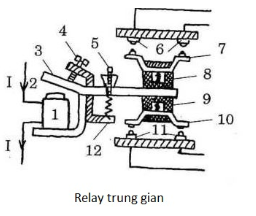
\includegraphics[width=0.5\textwidth]{pictures/NLHD_relay.png}
    \end{figure}
    \item Relay trung gian MY4N AC240/250, 14 chân, 5A (4PDT)
    \begin{figure}[H]
        \centering
        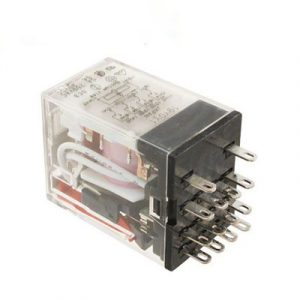
\includegraphics[width=0.5\textwidth]{pictures/Relay_4PDT.png}
    \end{figure}
    \item Relay trung gian MY2N AC240/250, 8 chân, 5A (DPDT)
    \begin{figure}[H]
        \centering
        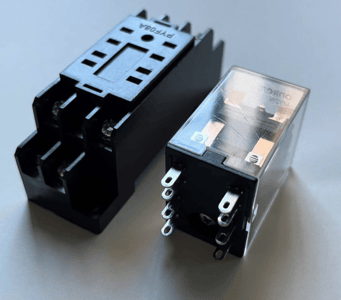
\includegraphics[width=0.5\textwidth]{pictures/Relay_DPDT.png}
    \end{figure}
\end{itemize}

\subsubsection{Module relay 4 kênh}
Module relay được sử dụng chung với cảm biến phát hiện kim loại. 
\begin{figure}[H]
    \centering
    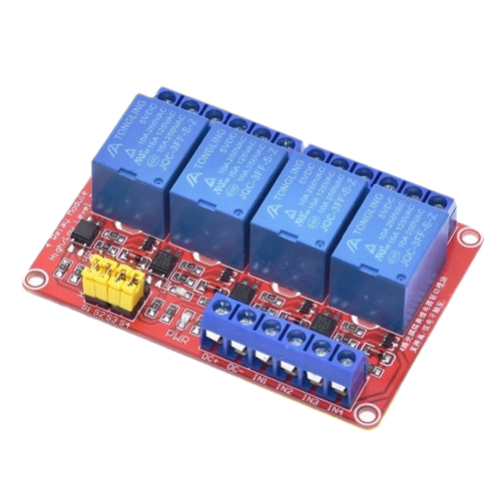
\includegraphics[width=0.5\textwidth]{pictures/Module_relay.png}
\end{figure}



\subsubsection{Cảm biến tiệm cận kim loại}
\begin{itemize}
    \item Cảm biến tiệm cận (Proximity Sensors). Còn có tên gọi khác là công tắc tiệm cận
    hay "PROX". Phản ứng khi có vật ở gần cảm biến.
    \item \textbf{Nguyên lý hoạt động:} Cảm biến tiệm cận NPN hoạt động dựa trên nguyên lý của 
    transitor NPN. Cấu tạo của cảm biến tiệm cận bao gồm 1 mạch phát hiện vật, mục đích để xử lí tín hiệu
    khi phát hiện vật gần cảm biến và chuyển đổi thành tín hiện điện cho mạch kế tiếp. Tiếp theo là 1 mạch ON/OFF NPN sử dụng tín hiệu
    điện từ mạch phát hiện vật để đóng ngắt transistor. Cuối cùng tín hiệu được xuất ra ngoài output (Output có thể là PLC, relay hoặc tải, \dots)
    \begin{figure}[H]
        \centering
        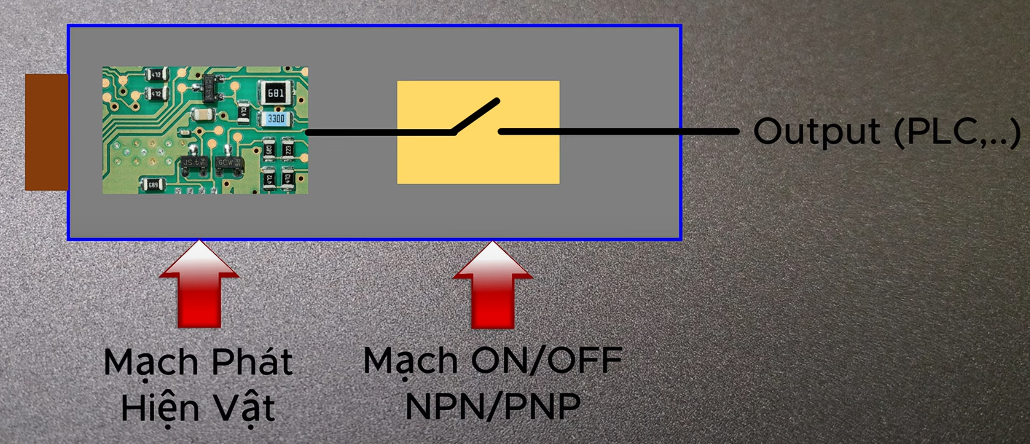
\includegraphics[width=0.7\textwidth]{pictures/structure_sensor.png}
    \end{figure}
    Cách đấu nối dây cho mạch sử dụng cảm biến tiệm cận kim loại NPN:
    \begin{figure}[H]
        \centering
        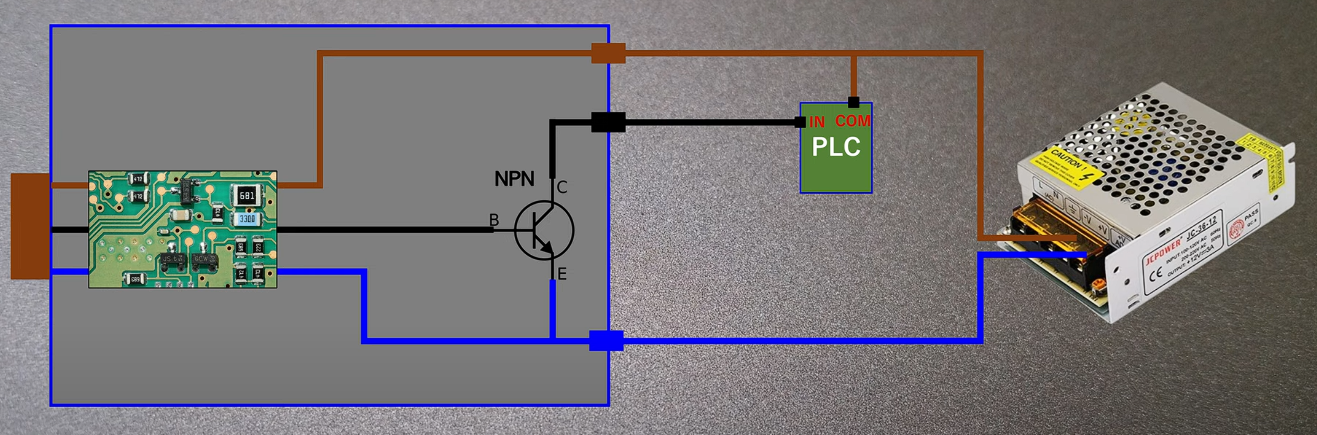
\includegraphics[width=1\textwidth]{pictures/mach_sensor.png}
    \end{figure}
    Trong trường hợp ở đây, chân tín hiệu của cảm biến sẽ được kết nối với module relay nhằm thực hiện nhiệm vụ như 1 công tắc trong mạch điều khiển
    ở các vị trí A1, B1, A2, B2.
\end{itemize}
Cảm biến phát hiện kim loại LJ12A3 loại NPN. 
\begin{figure}[H]
    \centering
    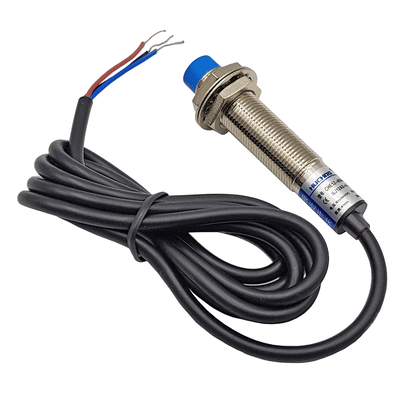
\includegraphics[width=0.5\textwidth]{pictures/Sensor.png}
\end{figure}
\cleardoublepage



\subsubsection{Động cơ}
Động cơ giảm tốc hộp số vuông góc JGY370 18RPM
\begin{figure}[H]
    \centering
    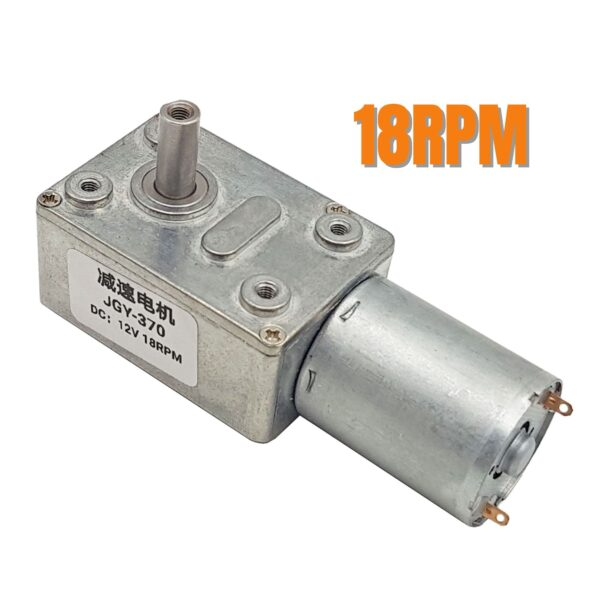
\includegraphics[width=0.5\textwidth]{pictures/motor.png}
\end{figure}

\cleardoublepage
    \section{Trình bày sơ đồ khối trong SFC}
Sơ đồ khối SFC  
\begin{figure}[H]
    \centering
    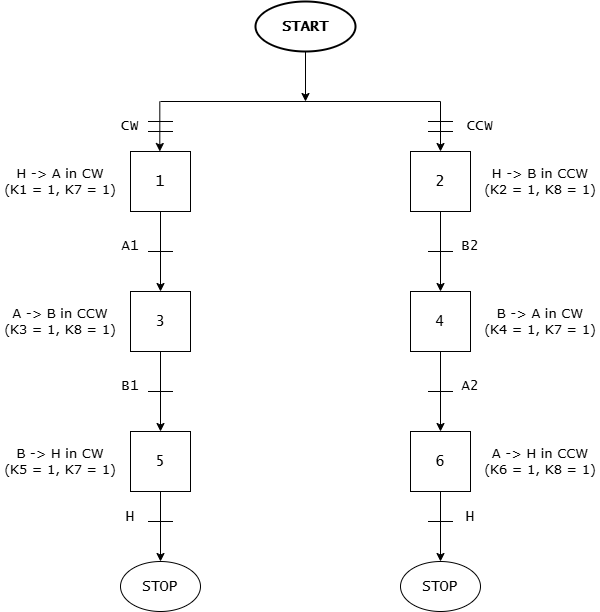
\includegraphics[width=0.9\textwidth]{pictures/SFC.png}
\end{figure}
Trong đó 2 nhánh lần lượt bắt đầu bằng CW, CCW thể hiện cho 2 nút bấm, 2 chế độ quay của bàn xoay.\\
Trong từng nhánh, các kí hiệu $Ki = 1 \,(i = 1, 2, \dots ,8)$ thể hiện trạng thái có điện của các cuộn dây $i$ tương ứng.
Trong đó $K7 = 1, \,K8 = 1$ lần lượt thể hiện cho chiều quay thuận và ngược chiều kim đồng hồ của động cơ.
\cleardoublepage
    \section{Triễn khai mạch điều khiển và mạch nguồn cho hệ thống}

\cleardoublepage
    \section{Mô tả hoạt động của hệ thống}

\cleardoublepage
\end{document}